% Copyright (c)  2005-2010 EDF-EADS-PHIMECA.
% Permission is granted to copy, distribute and/or modify this document
% under the terms of the GNU Free Documentation License, Version 1.2
% or any later version published by the Free Software Foundation;
% with no Invariant Sections, no Front-Cover Texts, and no Back-Cover
% Texts.  A copy of the license is included in the section entitled "GNU
% Free Documentation License".
\renewcommand{\filename}{docUC_StocProc_NormalProcess_Manipulation.tex}
\renewcommand{\filetitle}{UC : Manipulation of a stationary normal process}

% \HeaderNNIILevel
% \HeaderIILevel
\HeaderIIILevel


\index{Stochastic Process!Normal Process}

A stationary normal model is a particular process that proposes all the methods attached to a process : generate  a realization thanks to the method \emph{getRealization}, a sample of realizations thanks to the method \emph{getSample}. It is also possible to extract one marginal process, its time grid and get its dimension.\\

It is also possible to extract from the stationary normal process either its : 
\begin{itemize}
  \item its covariance model in case of a {\itshape TemporalNormalProcess} and then ask to the {\itshape CovarianceModel} thus generated to evaluate the covariance model  at the time stamps $(t,s)$ (or at $t-s$) thanks to the method \emph{computeCovariance} or discretize  the covariance model on a specific time grid thanks to the method \emph{discretizeCovariance} in order to get the matrix defined in (\ref{covMatrix});
  \item its spectral model in case of a {\itshape SpectralNormalProcess}  and then ask to the {\itshape SpectralModel} thus generated to evaluate the unilateral spectral density function $\mat{G}(f)$ defined in (\ref{univG}) at the frequence $f$ thanks to the method \emph{computeSpectralDensity}.
\end{itemize}

The first call to the method \emph{getRealization} implies different actions according to the type of thestationary  normal process : 
\begin{itemize}
  \item in case of a {\itshape TemporalNormalProcess}, Open TURNS builds the covariance matrix $\mat{C}_{1,\dots,n}$ defined in (\ref{covMatrix}) which is of size  ($nd \times nd$) with $n$ the size of the time grid and $d$ the dimension of the process, using  method \emph{discretizeCovariance}. Then $\mat{C}_{1,\dots,n}$ is factorized using the \emph{Cholesky} algorithm :  $\mat{C}_{1,\dots,n} = \mat{G} \, \mat{G}^{t}$. 
  \item in case of a {\itshape SpectralNormalProcess}, Open TURNS builds $n$ bilateral spectral density matrices $\mat{S}_{1,\dots,n}$ defined in (\ref{specdensFunc}) which are of size  ($d \times d$) with  $d$ the dimension of the process $n$ the number of discretized frequencies. Then $n$ matrices $\mat{S}_{1,\dots,n}$ are factorized using the \emph{Cholesky} algorithm :  $\mat{S}_{1,\dots,n} = \mat{H} \, \mat{H}^{t}$.
\end{itemize}
These matrices $\mat{G}$ or $\mat{H}$ are used to get some realizations of the process from realizations of a standard normal process (zero mean and unit covariance matrix). \\

In order to get the Cholesky factor of $\mat{C}_{1,\dots,n}$ or $\mat{S}_{1,\dots,n}$, we might need to scale the matrices, due to some numerical precisions. 
This scale consists in replacing the matrix $\mat{C}_{1,\dots,n}$ by 
$\mat{C}_{1,\dots,n}$ + $\epsilon * \mat{I}$ with  $\mat{I}$ the identity matrix and $\epsilon$ a negligible scalar variable. 
In this case, the User gets a warning message to inform him about the used $\epsilon$ value to get the Cholesky factor.\\

Details on each object may be found in the User Manual  (\href{OpenTURNS_UserManual_TUI.pdf}{see User Manual - Stochastic Process}).\\

 
\requirements{

  \begin{description}
  \item[$\bullet$] an normal process {\itshape myNormalProcess}
  \item[type:]  TemporalNormalProcess or  SpectralNormalProcess
  \end{description}

}
{

  \begin{description}
  \item[$\bullet$] a time series : {\itshape realization}
  \item[type:]  TimeSeries
  \end{description}

  \begin{description}
  \item[$\bullet$] a collection of time series : {\itshape sample}
  \item[type:]  ProcessSample
  \end{description}


  \begin{description}
  \item[$\bullet$] the graph : {\itshape myRealizationGraph}
  \item[type:]  Graph
  \end{description}
}

\textspace\\
Python script for this Use Case :

\begin{lstlisting}
   # Get the timeGrid
  myTimeGrid = myNormalProcess.getTimeGrid()

  # Realization using the time grid 
  realization = myNormalProcess.getRealization()x

  # Draw the realization  : marginal index 0
  myRealizationGraph = realization.drawMarginal(0)
  Show(myRealizationGraph)

  # Get a ProcessSample of k-realizations of the process
  sample = myNormalProcess.getSample(k)

  # Get the covariance model in case of TemporalNormalProcess
  myCovarianceModel = myNormalProcess.getCovarianceModel()
  
  # Compute the covariance matrix between the time stamps t and s
  covarianceMatrix = myCovarianceModel.computeCovariance(t,s)
  # or use the stationarity property
  covarianceMatrix = myCovarianceModel.computeCovariance(t-s)

  # Compute the discretization of the covariance model on the time grid myTimeGrid
  # The matrix is of size (nd) * (nd)
  discretizedCovariance = myCovarianceModel.discreteCovariance(myTimeGrid)

  # Get the sectral model in case of SpectralNormalProcess
  mySpectralModel = myNormalProcess.getSpectralModel()

  # Compute the unilateral spectral density G at frequency f
  unilatSpectralDensity = mySpectralModel.computeSpectralDensity(f)    
\end{lstlisting}

\textspace\\
The example illustrated below is a $2D$ Normal process with the Exponential model for the covariance one, parameterized by  $\vect{\lambda}=(1,1)$, $\vect{a}=(1,1)$ and $\mat{R}$ the identity matrix. We built a $TemporalNormalProcess$ and a $SpectralNormalProcess$ using the same $SecondOrderModel$ and the same $RegularGrid$. Figures (\ref{temporalNormalProcess_Realization}) to (\ref{spectralNormalProcess_Realizations}) respectively draw the graphs of : 
\begin{itemize}
  \item  one realization of the temporal process (both marginals are illustrated),
  \item   a sample of 5 realizations of the process (the first marginal is presented here) based on the covariance of the second order model, 
  \item  one realization of the spectral process (both marginals are illustrated), 
  \item  a sample of 5 realizations of the process (the first marginal is presented here) based on the spectral density of the second order model.
\end{itemize}

\begin{figure}[H]
  \begin{minipage}{9cm}
    \begin{center}
      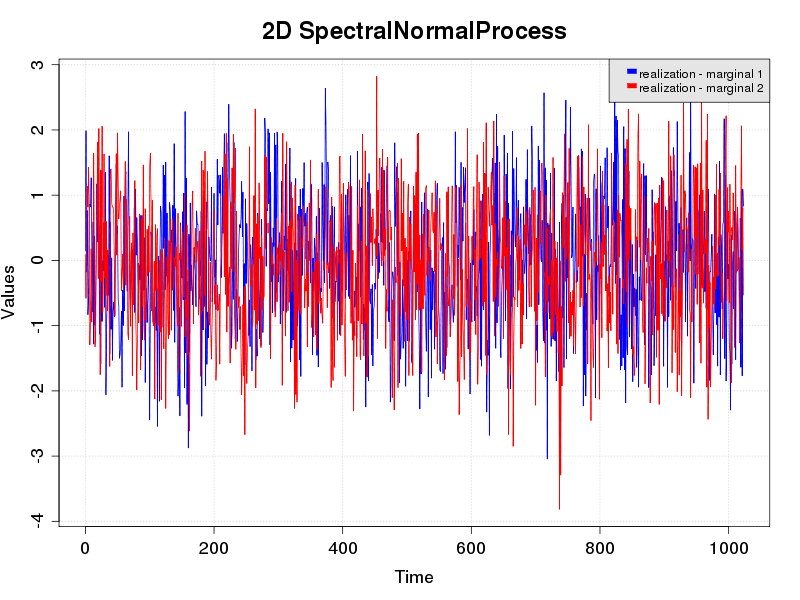
\includegraphics[width=7cm]{temporalNormal2D_realization.png}
      \caption{Realization of TemporalNormalProcess}
      \label{temporalNormalProcess_Realization}
    \end{center}
  \end{minipage}
  \hfill
  \begin{minipage}{9cm}
    \begin{center}
      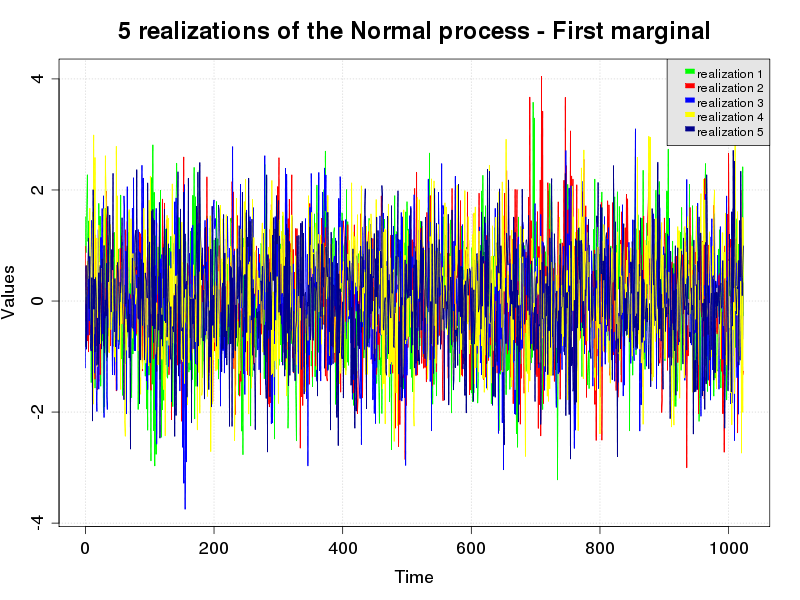
\includegraphics[width=7cm]{temporalNormal2D_realizations.png}
      \caption{$5$ realizations of the TemporalNormalProcess}
      \label{temporalNormalProcess_Realizations}
    \end{center}
  \end{minipage}
\end{figure}



\begin{figure}[H]
  \begin{minipage}{9cm}
    \begin{center}
      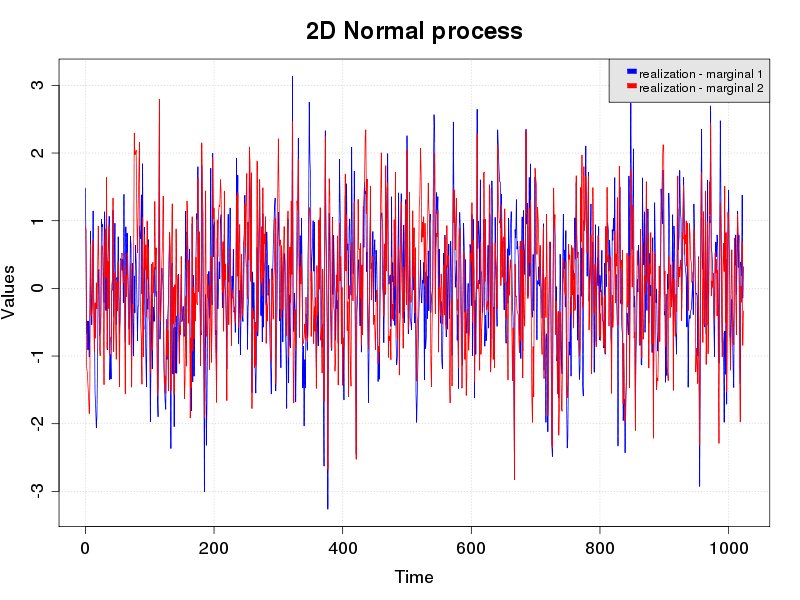
\includegraphics[width=7cm]{spectralNormal2D_realization.png}
      \caption{Realization of SpectralNormalProcess}
      \label{spectralNormalProcess_Realization}
    \end{center}
  \end{minipage}
  \hfill
  \begin{minipage}{9cm}
    \begin{center}
      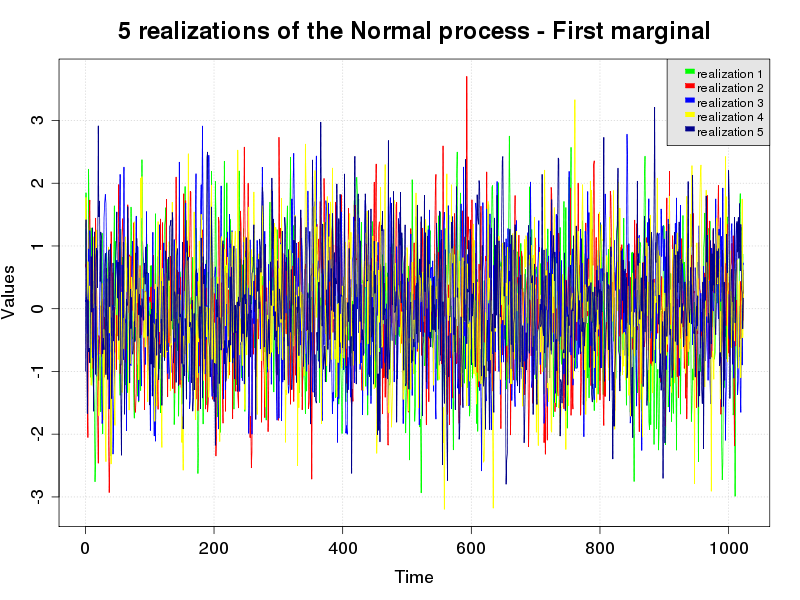
\includegraphics[width=7cm]{spectralNormal2D_realizations.png}
      \caption{$5$ realizations of the SpectralNormalProcess}
      \label{spectralNormalProcess_Realizations}
    \end{center}
  \end{minipage}
\end{figure}
